\chapter{FPGA}\label{chapter:fpga}

As this project requires us to implement a MIMD processor in VHDL, we realized
our design through implementing it in VHDL, and running the final processor on a
\todo{Replace ``Spartan-6'' and FPGA with references/links?}Spartan-6 FieldProgrammableGateArray.

Our MIMD processor design is was realized throughpipelined cores connected
sequentially in a pipeline of their own. Since the processor contains homogenous
cores, each core can receive and run the same instructions. To realize this as
an \todo{Fancy inline thingy explaining MultipleInstructionsMultipleData acronym}
``MIMD'', the first core in the sequential core-pipeline is the only one which
can work with the data given to said pipeline by the EBI bus. The next core then
works on the output of the first core, and in this fashion each core in the
pipeline works on its own data independently of the data any other core is
currently working on.

And each of the processor cores has its own instruction memory, so that they can
run each their own instructions, and that's how we have realized the \todo{Maybe add another fancy inline thingy here instead of qoutation marks?}
``Multiple Instruction'' part of the MIMD definition.

%Need something to insert a line here, or some other visual cue to cue the reader in that we're done with introducing the FPGA design, we're now going to tell the reader what to expect from the rest of the fpga chapter (I would prefer to use "\\"-x10)

This chapter is structured in the following manner; First, in section \ref{section:fpga-design}
we describe the design of the processor core in more detail, and explain the
reasoning behind the general design principles we followed. Second, in section \ref{section:sequential-pipeline}
we describe the aforementioned sequential pipeline in which the processor cores
are implemented. Third in section \ref{section:fpga-processor-core} we explain
the reasoning and design decisions behind the homogenous processor cores used
in the pipeline. Fourth, in section \ref{section:fpga-internal-memory} we
continue with describing the different types of memories that the processor as
a whole with all its cores utilize, from the instruction memory, to the data
memory, and the constant memory. Fifth, in section \ref{section:fpga-buses} we
describe how the processor this chapter so far has detailed communicates with
the MCU and the rest of the PCB through the EBI bus. Sixth, in section \ref{fpga-isa}
we list and describe how the assembly language the processor cores are
designed for works, as well as how it's meant to be utilized. Seventh, in
section \ref{section:fpga-testing} we conclude this chapter by explaining and
showing how the testing of the  \todo{Re-phrase this in a better way somehow?}
VHDL/FPGA implementation and methodology is discussed, including the subsequent
results.
\FloatBarrier
\section{Design Planning}\label{section:fpga-design}
\subsection{Design start}

As soon as it became decided that our project was going to aim for producing
some kind of ``sound-effect manipulating processor'', the group started looking
into how sound-effects were actually accomplished.

It quickly became apparent that for the most common, as well as the more
complicated effects, Fourier-transforms were crucial to the sound-manipulation
process. At least when sound manipulation was intended to run quickly enough,
as well as successfully on a computer processor.

This represented an (until now) unforeseen problem: Fourier-transforms are
algorithmically heavy in both time complexity and storage-space complexity,
which has the consequence that we would have to devote more of the FPGA
resources into circuits which could handle something as intensive as a
Fourier-transform. Especially if we wanted to perform these sound-effects in
real-time.

In effect, this revelation forced us to from a very early point to be
concerned about resource management on the FPGA.

\subsection{Fourier-transforms}\label{subsection:fpga-design-ft}

Looking into which types of Fourier-transform algorithms we could use on an
embedded device, in a manner as efficiently as possible, and yet real-time,
we ended up looking at Sliding-Discrete-Fourier-Transforms\cite{SD-FT} (or more
colloquially known as SD-FTs\footnote{This is discussed in more detail in
section \ref{subsubsection:fpga-alu-ft}.}).
\missingfigure{Maybe insert a figure here showing how the SD-FT works on each
sample at a time?}

This Fourier-transform would enable the FPGA to receive a live stream of
data samples representing sound from an input device through a mini-jack on the
PCB, or just from the DMAs of the MCU if the input was a file on a SD-card. And
then transform this live stream of samples into the frequency domain.

Since we now were able to work on each discrete sample while it was converted
into the frequency domain, we were now able to perform frequency based
sound-manipulations, such as basic high-pass and low-pass filters.

The sound-effect manipulations could now (in theory) be put to work.

\FloatBarrier
\subsection{Sequential processing cores?}\todo{Maybe find better subsection
title?}

Not all of the known sound-effects require (or are even possible) with a
Fourier-transform. Therefore it also became evident that for effects like say
the ``echo-effect'', we would need to do some post-processing after having
performed the inverse-Fourier-transform of the SD-FT\footnote{Sliding-Discrete
Fourier-transform, elaborated in the previous section
\ref{subsection:fpga-design-ft}.}.

Thus, so far this project required one processor-core to perform the SD-FT, and
another to perform the actual sound-effect done with the samples in the
frequency domain. A third core for the inverse SD-FT, and finally a fourth core
for any possible sound-manipulation that does not need a Fourier-transform (that
does not need to manipulate the data samples when converted into the frequency
domain).

With that reasoning in mind, we would need at least four processing cores, and
this for only one sound-channel. So for every additional sound-channel needed (
stereo needs two), we would have to add another four processor cores onto the
FPGA-chip.

It was decided early on to not settle for just one channel producing mono sound,
but to instead settle for at least two, so that we could listen to the output
on a stereo system. This let us then define the design for the processor
further, since it would need to have at the very least eight processor cores
implemented in some form of pipeline or other.

\subsection{Processing cores, 1-on-1}\todo{Maybe find better subsection title?}

Knowing we would need a minimum of eight processor cores on our FPGA processor,
and maybe more later down the line, we decided to start making things easier
for ourselves.

The decision was made to have all the cores homogenous, so that it would be
possible to send the same instructions to any core, being safe in the knowledge
that any core could perform said instructions.

This simplified the work in VHDL considerably, since we could then focus on
getting just \emph{one} processor core functioning, instead of say one
specifically for the SD-FT, another specifically tailored for the actual
sound-effects performed in the frequency domain, a third for the inverse-SD-FT,
and then the same as well for the fourth and final core performing the
``post-processing''. This would have (in all likelyhood) more than quadrupled
the amount of work required in VHDL for this project.

Due to all of the members in the FPGA-group taking the course TDT4255 \emph{
Computer Design} it may come as no surprise to any reader familiar with the
courses at IDI, NTNU, that this course was a big source of inspiration for the
development of our processor-core. Both the book\cite{tdt4255-book} and the
\emph{Computer Design} course were used as resources while developing the design
of this MIPS pipelined processor.

\subsection{Toplevel control register}\label{subsection:fpga-design-toplevel}


% !TEX root = ../../../report.tex
\FloatBarrier
\subsection{Audio Pipelines}\label{subsec:audio_pipelines}

\begin{figure}[H]
    \centering
    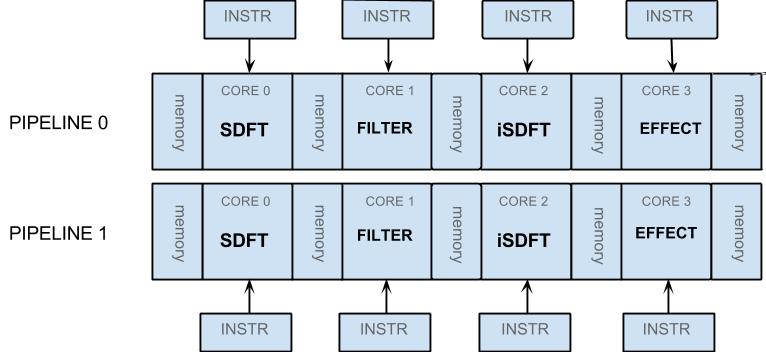
\includegraphics[height=150px]{figures/fpga/system_components_general_pipeline.png}
    \caption{Audio Pipeline Architecture}
    \label{fig:pipeline_architecture}
\end{figure}

\textit{ChaosM} consists of two audio processing pipelines, as illustrated in
Figure \ref{fig:pipeline_architecture}. These contain up to four processing cores
connected by data buffers. Each audio processing pipeline corresponds to one audio channel, operating on audio samples as elementary data elements.
The input/output frequency is directly tied to the sample rate of the input, which acts as a secondary clock input. The main system clock runs on the order of MHz, while this \textit{sample clk} is in the order of kHz and acts as a deadline for when new I/O is due.

\section{Processor Core}\label{section:fpga-processor-core}
\todo[inline]{How is the processor designed and \emph{why!}}

\FloatBarrier
\subsection{ALU}\label{subsection:fpga-alu}
\todo[inline]{ALU design and reasons why. -First revision finished?}

When the group sat down and started considering the ALU of our pipelined
processor cores, it was decided that we wanted to go for the ``Less is more''
design philosophy. This due to the fact that more often than not, the circuits
comprising the ALU logic tend to be the more resource-intensive and complicated
ones in a processor.

With that in mind, a following prioritization list of supported hardware
operations was made:\todo{This needs to be fleshed out when we've finished the
ALU.}
\begin{enumerate}
	\item Logic to allow for sufficiently fast Fourier-transforms (so that the
transform could be performed on each discrete sample within a single clockcycle
of the sequential processing core pipeline).
	\begin{enumerate}
		\item The Fourier-transform we settled on could be performed with only
addition, substraction, and shifting. Therefore hardware support for these
operations also had to be implemented.
	\end{enumerate}
	\item Multiplication for the sound-effect manipulations on the transformed
samples located in the frequency domain.
\end{enumerate}
\emph{For any reader potentially wondering, why division was left out, this is
explained in section \ref{subsubsection:fpga-alu-div}.}

\FloatBarrier
\subsubsection{Fourier-transforms}\label{subsubsection:fpga-alu-ft}
\todo[inline]{Need a way to refer to this subsubsection. I tried refering to it
in the design.tex file. The resulting reference refers to the ALU subsection as
a whole, and not the FT subsection.}

When it became necessary to start looking into how one implements a
Fourier-transform on a FPGA processor (as previously mentioned in section
\ref{section:fpga-design}), a lot of effort was spent on attemting to first find
examples of how others have implemented FT's (Fourier-transforms) on embedded
real-time devices before.

It did not take long before it became evident that there were two types of FT's
standing out from the rest of when considering FT's for the purpose of real-time
sound processing. Namely the Integer- and Sliding-Discrete- Fourier-Transforms.
The Integer-FT was ideal when considering that we would not have to implement
support for floating-point operations.

However, the Integer-FT needed the whole music file when transforming. It could
not transform discrete samples one at the time, which we would need if we had a
live source as input (say a portable music device connected to the PCB's
minijack). Also, we were unable to find any pseudo-code describing how such a
transform would function. The few examples we found described only the
mathematical functions, which left too huge a gap for us to research on our own.

Having found this out, the Sliding-Discrete-FTs potential use for our purposes
rose substantially. Not only would it allow us to perform a real-time
Fourier-transform, but we also managed to find pseudo-code describing how such a
transform would function. The big downside to the SD-FT however was the
necessity of floating-point to accomplish the implementation.

\FloatBarrier
\subsubsection{ALU input size}\todo{Better subsubsection title?}

Due to the algorithmically heavy operations of the SD-FT being the
\emph{heaviest} algorithmic operation performed in the the processor as a whole,
looking into how we could optimize the algorithm became a focus in the VHDL
group. Using the application \todo{Need references to actual (and correct!)
application notes here!}notes to find out the potential best speeds (read:
frequencies) of the FPGA, we then started calculating how fast the SD-FT would
have to perform its transform per sample.

It quickly became apparent that a ``quick and easy'' way to drastically reduce
the time complexity the algorithm would need to transform each sample, was to
reduce the sample sizes. \todo[inline]{Find some reference, or picture, or add a
paragraph explaining said algorithm.}With this in mind, we started testing how
small samples we could have, and yet have a passable level of sound quality. The
final result we ended up on was to have eight-bit datasamples. This had the
consequence of reducing the maximum sound frequency from ca. 44 kilohertz down
to \todo{This needs to be confirmed/edited.}11.

\FloatBarrier
\subsubsection{Leaving out division}\label{subsubsection:fpga-alu-div}

The decision to not implement hardware support for division was done for several
reasons. Firstly, hardware support for division is costly. Secondly, seeing as
we had already decided on having to implement floating-point for the SD-FT, we
decided that the amount of logic needed for each core to support both division
and floating-point was too much. Thirdly, having floating-point support, we
just as well multiply with a number smaller than one to perform a division. For
integer division it was decided that the programmer could program the cores to
perform longdivision with addition and substraction loop (or shifting when a
division by a power of 2 was attempted).


\subsection{Floating-point implementation design choices}

\subsection{Datapath/pipelining of the core}
\todo[inline]{Describe the pipelines of the cpu, and why it is implemented/
designed the way it is.}

\subsection{Memory access}
\todo[inline]{Why constant values go to the alu, and how it changes pipeline
layout. How the core accesses memory.}
\section{Internal memory\todo{Better title}}\label{section:fpga-internal-memory}
\todo[inline]{Should contain: Ringbuffer, Switch buffer, input/output buffers,
constant memory, inst memory, read and write lines to the fpga from the ARM.
Originally the ARM only needed access to the first and the last data buffer but
for debugging purposes the ARM was given access to all buffers.}
\todo[inline]{Short description? Discuss non-uniform memory access and important
things.}

\subsection{Intruction memory}
\todo[inline]{Describe the functionality and reasons behind decisions regarding
the instruction memory. -First revision done. Finished?}

The instruction memory for each core is how we realize the ``Multiple
Instructions'' part of the ``MIMD'' definition. This instruction memory which
each core has is how the separate cores can run each their own independent
instructions.

Due to the manner in which this system is intended to be intialized (as detailed
in section \ref{subsection:fpga-pipeline-startup}), another aspect of this
implementation choice is that before starting up all the cores (in effect
starting up the sequential pipelines), the MCU must through the EBI-bus write
the instructions into this instruction memory in each core, and in this manner
set up which core in the sequential pipelines is supposed to perform which job.

\subsection{Processor input/output memory}\label{subsection:fpga-internmem-IO}
\todo[inline]{Describe the need for memory to behave as both ringbuffer/queues,
and as switching buffers. Discuss why this is a good idea because of our
intended functionality, and how we utilize the FPGAs resources to implement it
in the best possible way.}

\subsection{Pipeline constant memory}
\todo[inline]{Why did we separate this from input/ouput memory? Why is it shared
between cores, and how? The reason we send it's values directly to the alu
instead of to the register file?}
\FloatBarrier
\section{Communication}

\subsection{The External Bus Interface}
The microcontroller communicates with the FPGA design using the External Bus
Interface (EBI) of the Giant Gecko microcontroller. The EBI is a parallel bus
with a separate data and address bus in addition to the chip select and read and
write enable signals, all active low\cite{efm_ebi}.

The communication between the MCU and the FPGA uses 23 address lines and 16
data lines. All transfers are initiated by the chip select signal going low.
Then, for write transfers, the data and address lines are set up and the
write enable signal is asserted, see figure \ref{fig:ebi_write}. For reads,
the address is set up and the data line is put in high impedance mode before
the read enable signal is asserted, see figure \ref{fig:ebi_read}.

\begin{figure}[h]
	\centering
	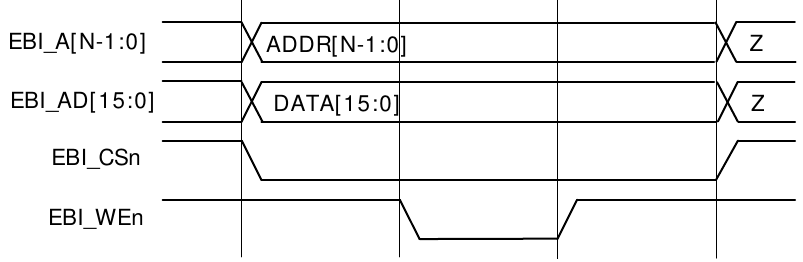
\includegraphics[width=0.8\linewidth]{figures/fpga/ebi_write.png}
	\caption{EBI write transfer\cite[p.6]{efm_ebi}}
	\label{fig:ebi_write}
\end{figure}



\begin{figure}[h]
	\centering
	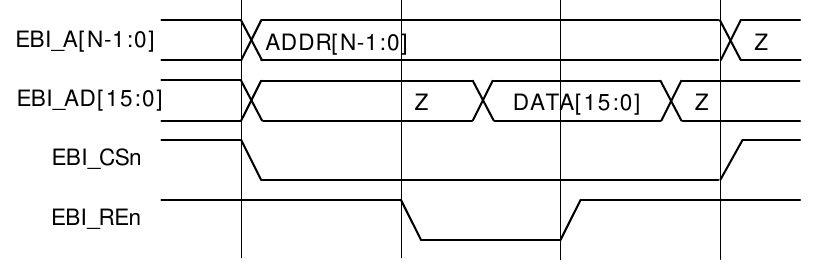
\includegraphics[width=0.8\linewidth]{figures/fpga/ebi_read.png}
	\caption{EBI read transfer\cite[p.7]{efm_ebi}}
	\label{fig:ebi_read}
\end{figure}



\FloatBarrier
\subsection{The Internal Bus}

The internal bus is used to transfer data to and from modules in the FPGA.
All transfers are initiated by the microcontroller on the EBI bus, and the
EBI controller module translates between the EBI and the internal bus.

\subsubsection{The EBI controller}
The EBI controller module is used to handle EBI transfers initiated by the
microcontroller. It consists of a simple state machine, illustrated in
figure \ref{fig:ebi_ctrl_fsm}. When an EBI transfer is executed, the
internal bus, described in is used to store or retrieve data from a module
in the FPGA.

In the idle state, the EBI data lines are set as high impedance, which
causes the microcontroller to have control of the data bus. Only when
a value is read over the EBI bus, does the EBI controller take control of
the data lines.

To save power, a clock gate is used to turn off the functional clock to
the EBI controller when the chip select signal is deasserted.

\begin{figure}[h]
	\centering
	% TODO: Make the arrows in separate directions be separate arrows
	\begin{tikzpicture}[shorten >= 1pt,node distance=2cm,on grid,auto]
		\node[state,initial] (idle) {idle};
		\node[state] (read) [above right=of idle] {read};
		\node[state] (write) [below right=of idle] {write};
		\path[->]
			(idle) edge node {\small RE = 0} (read)
			       edge node [swap] {\small EW = 0} (write)
			(read) edge node {\small RE = 1} (idle)
			(write) edge node [swap] {\small WE = 1} (idle);
	\end{tikzpicture}
	\caption{EBI controller state machine}
	\label{fig:ebi_ctrl_fsm}
\end{figure}




\subsubsection{Addressing}

Modules in the FPGA is addressed using a simple hierarchical scheme, where the
address is divided into three parts; the pipeline where the module is located,
the ``index'' of the module and an address specifying where in the module to
read or write data. Figure \ref{fig:ebi_addresses} illustrates the address
format.

\begin{figure}[H]
	\centering
	\begin{bytefield}[endianness=big,bitwidth=0.04\linewidth]{23}
		\bitheader{0-22}\\
		\bitbox{1}{T} &
		\bitbox{2}{\tiny Pipeline} &
		\bitbox{4}{Device} &
		\bitbox{2}{\tiny Subdev} &
		\bitbox{14}{Address}
	\end{bytefield}
	\caption{FPGA address format}
	\label{fig:ebi_addresses}
\end{figure}




\FloatBarrier
\subsubsection{Read Transfers}

A read transfer is initiated when the read enable line from the microcontroller goes low.
The EBI controller sets up the internal address signals and asserts the internal read enable
signal. This causes the requested data to be available in the next clock cycle. The EBI
controller switches to read state, where it remains until the read enable signal is deasserted.

\subsubsection{Write Transfers}

Write transfers are initiated the same way as read transfers. As the write-enable signal goes
low, the destination address is latched into the internal address bus and the internal data
lines are set to the value of the EBI data lines. The internal write enable signal is asserted
and the EBI controller enters the write state. In the write state the internal write enable
signal is reset, and when the EBI write enable signal is deasserted, idle mode is reentered.


% !TEX root = ../../../report.tex
\subsection{Instruction Set Architecture}\label{section:fpga-isa}

The processor was designed in a top-down fashion, starting with the instruction
set. The MIPS ISA used in the \textit{Computer
Design}\cite{tdt4255} course was a good starting point for the ISA used in this
project. In order to support as many different filters
and effects as possible, the processor supports all normal arithmetic
operations. Due to the requirements of doing Fourier transforms on the
processor, support for some floating point instructions was also included.

To make the decoding of instructions as easy as possible, instructions
were divided into three different instruction groups.

\subsubsection{Register-based Instructions}

The register-based instructions are instructions were both operands are
primarily registers. The group also includes a few instructions where
the second operand is an immediate value. The format of the
instructions are illustrated in Figure \ref{fig:regbased_instrs_format}. The
implemented functions can be found in Table \ref{tab:regbased_instrs}.

\begin{figure}[h]
	\centering
	\begin{bytefield}[bitwidth=0.05\linewidth]{16}
		\bitheader{0-15}	\\
		\bitbox{2}{Group}	&
		\bitbox{2}{Funct}	&
		\bitbox{2}{Opt}		&
		\bitbox{5}{Reg A}	&
		\bitbox{5}{Reg B/Imm}
	\end{bytefield}

	\caption{Register-based instruction format}
	\label{fig:regbased_instrs_format}
\end{figure}

\FloatBarrier
\begin{table}[H]
	\centering
	\begin{tabular}{|l l l l l|}
		\hline
		\textbf{Funct} & \textbf{Opt}  & \textbf{Mnemonic} & \textbf{Instruction} & \textbf{Operation} \\
	\hline
	\multicolumn{5}{|c|}{Group \texttt{0b00}} \\
	\hline
	\multirow{3}{*}{\texttt{0b00}}
		& \texttt{0b00} & \texttt{add \$ra, \$rb}  & Add registers & $\$ra \leftarrow \$ra + \$rb$ \\
		& \texttt{0b01} & \texttt{addi \$ra, imm} & Add immediate & $\$ra \leftarrow \$ra + imm$ \\
		& \texttt{0b10} & \texttt{fadd \$ra, \$rb} & Add registers (FP) & $\$ra \leftarrow \$ra + \$rb$ \\
	\multirow{4}{*}{\texttt{0b01}}
		& \texttt{0b00} & \texttt{sub \$ra, \$rb}  & Subtract registers & $\$ra \leftarrow \$ra - \$rb$ \\
		& \texttt{0b01} & \texttt{fsub \$ra, \$rb} & Subtract registers (FP) & $\$ra \leftarrow \$ra - \$rb$ \\
		& \texttt{0b10} & \texttt{cmp \$ra, \$rb}  & Compare & $cnd \leftarrow cnd(\$ra - \$rb)$ \\
		& \texttt{0b11} & - & compare fp / subtract imm? & - \\
	\multirow{4}{*}{\texttt{0b10}}
		& \texttt{0b00} & \texttt{mul \$ra, \$rb}  & Multiply registers & $\$ra \leftarrow \$ra * \$rb$ \\
		& \texttt{0b01} & \texttt{fmul \$ra, \$rb} & Multiply registers (FP) & $\$ra \leftarrow \$ra * \$rb$ \\
		& \texttt{0b10} & \texttt{fmla \$ra, \$rb} & Multiply-and-accumulate (FP) & $\$ra \leftarrow \$ra + \$rb * \$rc$ \\
		& \texttt{0b11} & \texttt{fmls \$ra, \$rb} & Multiply-and-subtract (FP) & $\$ra \leftarrow \$ra - \$rb * \$rc$ \\
	\multirow{2}{*}{\texttt{0b11}}
		& \texttt{0b00} & \texttt{shl \$ra, imm} & Shift left & $\$ra \leftarrow \$ra << imm$ \\
		& \texttt{0b01} & \texttt{shr \$ra, imm} & Shift right & $\$ra \leftarrow \$ra >> imm$\\
	\hline
	\multicolumn{5}{|c|}{Group \texttt{0b01}} \\
	\hline
	\multirow{2}{*}{\texttt{0b00}}
		& \texttt{0b00} & \texttt{and \$ra, \$rb} & And & $\$ra \leftarrow \$ra \wedge \$rb$ \\
		& \texttt{0b01} & \texttt{nand \$ra, \$rb} & Nand & $\$ra \leftarrow \neg(\$ra \wedge \$rb)$ \\
	\multirow{3}{*}{\texttt{0b01}}
		& \texttt{0b00} & \texttt{or \$ra, \$rb} & Or & $\$ra \leftarrow \$ra \vee \$rb$ \\
		& \texttt{0b01} & \texttt{nor \$ra, \$rb} & Nor & $\$ra \leftarrow \neg(\$ra \vee \$rb)$\\
		& \texttt{0b10} & \texttt{xor \$ra, \$rb} & Xor & $\$ra \leftarrow \$ra \oplus \$rb$\\
	\multirow{4}{*}{\texttt{0b10}}
		& \texttt{0b00} & \texttt{mov \$ra, \$rb} & Move & $\$ra \leftarrow \$rb$\\
		& \texttt{0b01} & \texttt{mvn \$ra, \$rb} & Move negative & $\$ra \leftarrow \neg\$rb$ \\
		& \texttt{0b10} & \texttt{i2f \$ra, \$rb} & Typecast (Int to FP) & $\$ra \leftarrow fp(\$rb)$ \\
		& \texttt{0b11} & \texttt{f2i \$ra, \$rb} & Typecast (Fp to int) & $\$ra \leftarrow int(\$rb)$ \\
	\multirow{4}{*}{\texttt{0b11}}
		& \texttt{0b00} & \texttt{lda \$ra, [\$rb]} & Load from input & $\$ra \leftarrow [\$rb]$ \\
		& \texttt{0b01} & \texttt{ldb \$ra, [\$rb]} & Load from output & $\$ra \leftarrow [\$rb]$ \\
		& \texttt{0b10} & \texttt{ldc \$ra, [\$rb]} & Load from constant buffer & $\$ra \leftarrow [\$rb]$ \\
		& \texttt{0b11} & \texttt{stb \$ra, [\$rb]} & Store to output & $[\$rb] \leftarrow \$ra$ \\
	\hline
	\end{tabular}
	\caption{Register-based instruction list}
	\label{tab:regbased_instrs}
\end{table}


\FloatBarrier

\subsubsection{Load Immediate Instruction}
The load immediate instruction is used to load an immediate constant into a
register. The format of the instruction can be found in figure
\ref{fig:ldi_format}. The value is loaded into register \texttt{\$r1}.

\begin{figure}[h]
	\centering
	\begin{bytefield}[bitwidth=0.05\linewidth]{16}
		\bitheader{0-15} \\
		\bitbox{2}{Group} &
		\bitbox{14}{Imm}
	\end{bytefield}

	\caption{Load immediate format}
	\label{fig:ldi_format}
\end{figure}

\FloatBarrier

\subsubsection{Branch Instruction}
The branch instruction checks condition flags and jumps accordingly. By
checking for various combinations of the condition flags, many different
conditions can be checked for. The format of the instruction is illustrated
in Figure \ref{fig:new_branch_format}.

\begin{figure}[h]
	\centering
	\begin{bytefield}[bitwidth=0.05\linewidth]{16}
		\bitheader{0-15} \\
		\bitbox{2}{Group} &
		\bitbox{4}{Flags} &
		\bitbox{11}{Target}
	\end{bytefield}

	\caption{Branch instruction format}
	\label{fig:new_branch_format}
\end{figure}


\FloatBarrier

\paragraph{Special Registers}

Due to the limited space in instruction words, only two registers at most can be
specified in an instruction. Some instructions, such as the load immediate and
load constant instructions do not specify any registers, only an immediate
offset constant.

The list of defined special registers can be found in Table \ref{tab:specregs}.

\begin{centering}[h]
	\begin{tabular}{|l p{10.5cm}|}
		\hline
		\textbf{Register name} & \textbf{Register purpose} \\
		\hline
		\texttt{r0} & Zero register, hard coded to always contain 0 \\
		\texttt{r1} & Immediate register, contains the result of an \textsc{ldi} instruction\\
		\texttt{rc} & Constant register, provides operand to \textsc{fmla} and \textsc{fmls} instructions. Lies within the ALU. \\
		\texttt{rc} & Constant register, provides operand to \textsc{fmla} and \textsc{fmls} instructions. Lies within the ALU. \\
		\hline
	\end{tabular}

	\label{tab:specregs}
	%\caption{List of special registers}
	
\end{centering}


\FloatBarrier

\section{Testing the FPGA}\label{section:fpga-testing}

\subsection{FPGA prototype}
\todo[inline]{How we tested that the FPGA was soldered onto the PCB. Can move this section.}

\subsection{Testing the processor design}
\todo[inline]{Testing methodology}

\subsection{Simulation}
\todo[inline]{Simluation description}

\subsubsection{Tests\todo{insert more of these, along with descriptions and reasons.}}

\subsection{Integrated tests}
\todo[inline]{Description of testing on board}

\subsubsection{Tests\todo{insert more of these, along with descriptions and reasons.}}


